% Optimization Project: Biscuit Optimizer
% Roberto Basla
% Politecnico di Milano
% A.Y. 2021/2022

\section{Conclusions}

This project implemented models and heuristics in order to solve the nesting problem of biscuit cutters given the available cookie dough. Due to the NP-Hard nature of this class of problems, optimization models were not able to find the optimal solution in a reasonable time; the devised heuristics, especially in the case of GRASP with Path Relinking, were able to outperform the models' partial results. Table \ref{tab:final_results} reports the best values for each of the technologies and strategies described in this report, while Figure \ref{fig:best_solution} displays the best solution found.

\begin{center}
	\begin{tabular}{r|c|c|c}
		Problem				& Technology / Algorithm	& Best value	& Time		\\
		\hline
		Integer Knapsack	& AMPL (CPLEX)           	& 29000      	& 0.11		\\  
		Integer Knapsack 	& OR-Tools (CP-SAT)      	& 29000      	& 0.562 	\\  
		Integer Knapsack	& Gurobi                 	& 29000      	& 0.2   	\\
		Nesting				& AMPL (CPLEX)           	& 16300      	& 40000 	\\
		Nesting				& OR-Tools (CP-SAT)      	& 17800      	& 40000 	\\
		Nesting				& Gurobi                 	& 17800      	& 40000		\\
		Nesting				& Greedy heuristics      	& 16900      	& 3.45   	\\
		Nesting				& GRASP                  	& 17800      	& 317.77	\\
		Nesting				& GRASP (Path Relinking) 	& 18500      	& 2765.12      
	\end{tabular}
	\captionof{table}{\label{tab:final_results}Final results for each problem and solution}
\end{center}

\begin{figure}[H]
	\begin{subfigure}[b]{.49\textwidth}
		\centering
		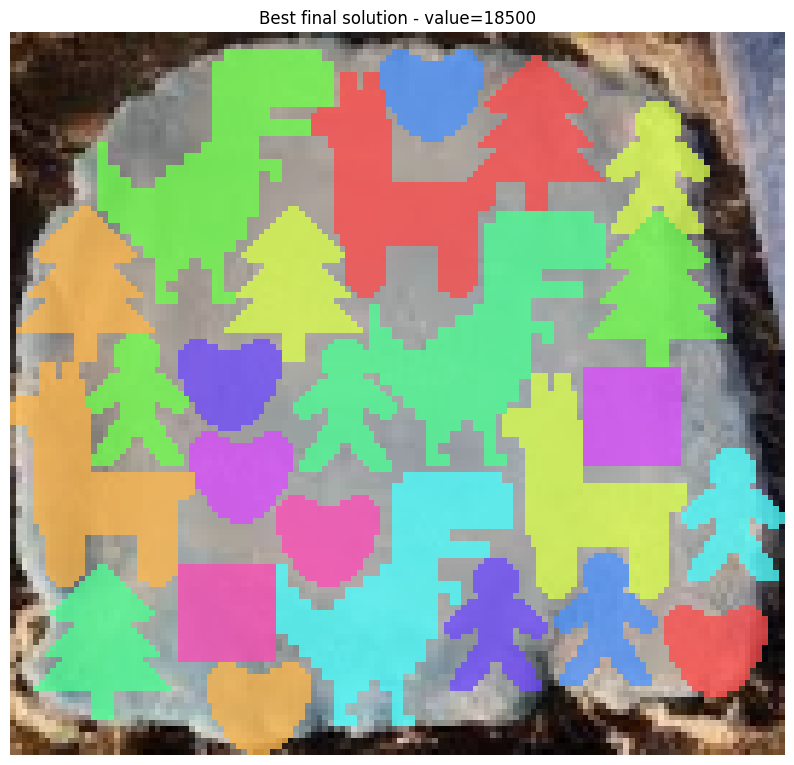
\includegraphics[width=\textwidth]{05-conclusions/best_dough}
		\caption{Best solution placement}
		\label{fig:best_dough}
	\end{subfigure} 
	\hfill
	\begin{subfigure}[b]{.49\textwidth}
		\centering
		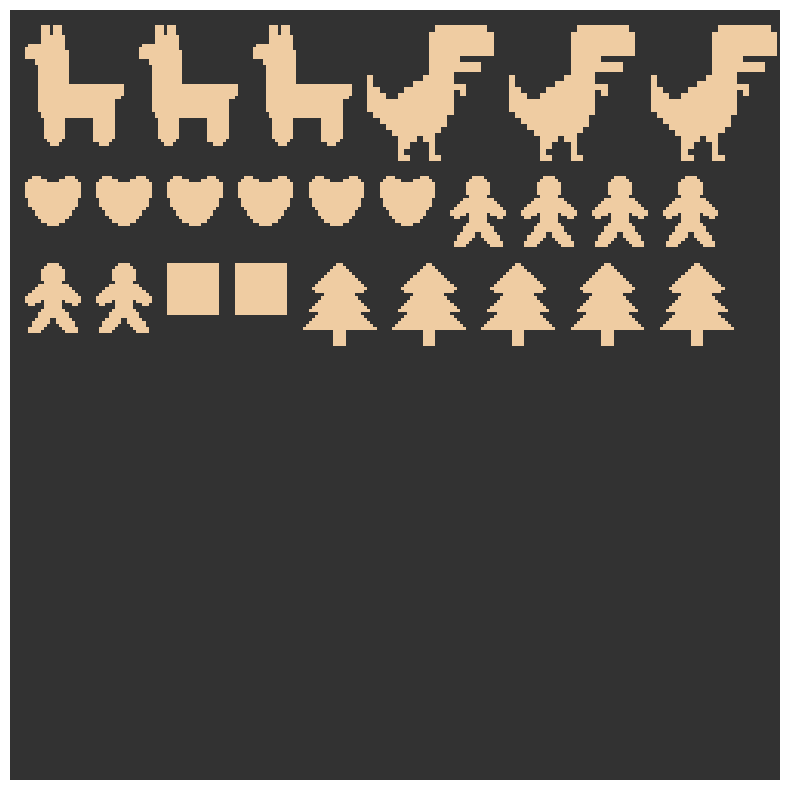
\includegraphics[width=\textwidth]{05-conclusions/best_pan}
		\caption{Best solution biscuits result}
		\label{fig:best_pan}
	\end{subfigure}
	\caption{Best solution}
	\label{fig:best_solution}
\end{figure}
